%!TEX encoding = UTF-8 Unicode
% ================================================================================

\documentclass[
    fontsize=12pt,
    headings=small,
    parskip=half,           % Ersetzt manuelles Setzen von parskip/parindent.
    bibliography=totoc,
    numbers=noenddot,       % Entfernt den letzten Punkt der Kapitelnummern.
    open=any,               % Kapitel kann auf jeder Seite beginnen.
%   final                   % Entfernt alle todonotes und den Entwurfstempel.
    ]{scrreprt}
%\usepackage[backend=biber,
%style=alphabetic,
%]{biblatex}
% ===================================Praeambel==================================
% Kodierung, Sprache, Patches {{{
\usepackage[T1]{fontenc}    % Ausgabekodierung; ermöglicht Akzente und Umlaute
                            %  sowie korrekte Silbentrennung.
\usepackage[utf8]{inputenc} % Erlaubt die direkte Eingabe spezieller Zeichen;
                            %  utf8 muss die Eingabekodierung des Editors sein.
\usepackage[english]{babel} 
\usepackage{microtype}      % Optimale Randausrichtung und Skalierung.


%\usepackage[
%    autostyle,
%    ]{csquotes}             % Korrekte Anführungszeichen in %der Literaturliste.
%\usepackage{fixltx2e}      % Patches fuer LaTeX2e - seit 2015 nicht mehr nötig
\usepackage{scrhack}        % Verhindert Warnungen mit älteren Paketen.
\usepackage[
  newcommands
]{ragged2e}                 % Verbesserte \ragged...Befehle
\PassOptionsToPackage{
  hyphens
}{url}                      % Sorgt für URL-Umbrüche in Fußzeilen u. Literatur
% }}}

% Schriftarten {{{
\usepackage{mathptmx}       % Times; modifies the default serif and math fonts
\usepackage[scaled=.92]{helvet}% modifies the sans serif font
\usepackage{courier}        % modifies the monospace font
% }}}

\usepackage{comment}

% Biblatex {{{
%\usepackage[
%    style=alphabetic,
%    backend=biber,
%    backref=true
%    ]{biblatex}             % Biblatex mit alphabetischem %Style und biber.
%\bibliography{bibliography} % Dateiname der bib-Datei.
%\DeclareFieldFormat*{title}{
%    \mkbibemph{#1}}         % Make titles italics
% }}}

% Dokument- und Texteinstellungen {{{
\usepackage[
    a4paper,
    margin=2.54cm,
    marginparwidth=2.0cm,
    footskip=1.0cm
    ]{geometry}             % Ersetzt 'a4wide'.
\clubpenalty=10000          % Keine Einzelzeile am Beginn eines Absatzes
                            %  (Schusterjungen).
\widowpenalty=10000         % Keine Einzelzeile am Ende eines Absatzes
\displaywidowpenalty=10000  %  (Hurenkinder).
\usepackage{floatrow}       % Zentriert alle Floats
\usepackage{ifdraft}        % Ermöglicht \ifoptionfinal{true}{false}
\pagestyle{plain}           % keine Kopfzeilen
% \sloppy                    % großzügige Formatierungsweise
\deffootnote{1em}{1em}{
  \thefootnotemark.\ }      % Verbessert Layout mehrzeiliger Fußnoten

\makeatletter
\AtBeginDocument{%
    \hypersetup{%
        pdftitle = {\@title},
        pdfauthor  = \@author,
        pdfsubject = \@subject,
        pdfproducer = \@producer,
    }
}
\makeatother
% }}}




% Weitere Pakete {{{
\usepackage{graphicx}       % Einfügen von Graphiken.
\usepackage{tabu}           % Einfügen von Tabellen.
\usepackage{multirow}       % Tabellenzeilen zusammenfassen.
\usepackage{multicol}       % Tabellenspalten zusammenfassen.
\usepackage{booktabs}       % Schönere Tabellen (\toprule\midrule\bottomrule).
\usepackage[nocut]{thmbox}  % Theorembox bspw. für Angreifermodell.
\usepackage{amsmath}        % Erweiterte Handhabung mathematischer Formeln.
\usepackage{amssymb}        % Erweiterte mathematische Symbole.
\usepackage{rotating}
\usepackage[
    printonlyused
    ]{acronym}              % Abkürzungsverzeichnis
\usepackage[
    colorinlistoftodos,
    textsize=tiny,          % Notizen und TODOs - mit der todonotes.sty von
    \ifoptionfinal{disable}{}%  Benjamin Kellermann ist das Package "changebar"
    ]{todonotes}            %  bereits integriert.
\usepackage{hyperref}
\hypersetup{
    colorlinks=true,
    linkcolor=black,
    filecolor=black,  
    citecolor=black,
    urlcolor=blue,
    
    
}

%\usepackage[
%    breaklinks,
%    pdfdisplaydoctitle,
%    pdfpagemode = {UseOutlines},
%    pdfpagelabels,
%    ]{hyperref}             % Sprungmarken im PDF. Lädt das URL-Paket.
    % \urlstyle{rm}           % Entfernt die Formattierung von URLs.
%\usepackage{breakurl}
%\def\UrlBreaks{\do\/\do-}
\usepackage{listings}       % Spezielle Umgebung für Quelltextformatierung.
    \lstset{                
        language=C,
        breaklines=true,
        breakatwhitespace=true,
        frame=l,            % Linie links: l, doppelt: L
		framerule=2.5pt,    % Dicke der Linie
		rulecolor=\color{gray},% Farbe der Linie
        captionpos=b,
        xleftmargin=6ex,
        tabsize=4,
        numbers=left,
        numberstyle=\ttfamily\footnotesize,
        basicstyle=\ttfamily\footnotesize,
        keywordstyle=\bfseries\color{green!50!black},
        commentstyle=\itshape\color{magenta!90!black},
        identifierstyle=\ttfamily,
        stringstyle=\color{orange!90!black},
        showstringspaces=false,
        }
%\usepackage{filecontents}  % Direktes Einfügen von Dateiinhalt. Wird hier für
                            %  die Verwendung einer .bib-Datei in dieser .tex-
                            %  Datei benötigt.
% }}}

\usepackage{biblatex}
\addbibresource{Report_Covid_19/bibliography.bib}
\usepackage{csquotes}


% ===================================Dokument===================================

\title{COVID-19 Sentiment Analysis}
\author{\\ Christoph Koenning, Hamed Mohammadi, Johannes Idelberger, Lukas Oberfrank}

\date{April 2021} % Falls ein bestimmtes Datum eingesetzt werden soll, einfach
                    %  diese Zeile aktivieren.

\begin{document}

\begin{titlepage}

\includegraphics[width=6.8cm]{../pic/up-uhh-logo-u-2010-u-farbe-u-rgb.pdf}
\begin{center}\Large
    % Universität Hamburg \par
    % Fachbereich Informatik
    \vfill
    \makeatletter
    {\Huge\textsf{\textbf{\@title}}\par}
    \par
    \makeatother
    \bigskip
    base.camp Praktikumsbericht \par
    \bigskip
    \makeatletter
    Authors: {\@author} \par
    \makeatother
    \bigskip
    Examiner: Eugen Ruppert \par
    \bigskip
    \bigskip
    \makeatletter
    {\@date}
    \makeatother
    
    \makeatother
    \vfill
    \vfill
    %(Muster für das Deckblatt: siehe Anhang dieser Hinweise)
\end{center}
\end{titlepage}





\tableofcontents


\chapter{Overview of the project}


\section{Project description}

This project deals with the social media analysis of data concerning COVID-19. Individual problem sectors are to be analyzed concerning their suitability for COVID-19 and filtered out using Big Data tools like MapReduce, Apache Hadoop, or TextBlob. In particular, we want to find out to what extent the people's sentiment regarding COVID-19 differs every month and any significant correlations. The data set will be limited to Germany.


\\
This analysis is particularly well suited for presenting complex interrelationships in business, society and administration in a compact way. Empathy and understanding for individual events can also be stimulated. To realize this we searched for ideas that could easily display the complexity that the problem definition comes along with in an easy to understand prototype. In order to be able to check the prototype for correctness, testing plays an important role in order to be able to adapt improvements and suggestions before the release and thus deliver correct data.

\section{Project objectives}
The goal of this project is to understand a connection and correlation between the sentiment of Tweets concerning COVID-19 and the political environment and political measures (e.g., lockdowns) in Germany in 2020.
To reach this goal, a sentiment analysis was conducted on basis of a 900GB dataset of Twitter data from 2020. The data was then stored in a external data base and visualized by several charts to provide comprehensible information to the user.
\\


\chapter{Organization and planning}

This section presents the organization and planning of the project in a descriptive way and shows how we proceeded with our organization to meet our project goals as satisfactorily as possible in the appropriate time.\\
Section 1 presents our modes of communication, which were limited to online resources due to the pandemic.
In the second section, we look at individual days and describe in detail what our individual milestones were in terms of setting goals. Section 3 presents a concrete method of project management, the Daily Scrum, and shows how we used this for our project fulfillment. The last section discusses how GitHub was able to help us achieve good coordination despite being remote.
\section{Communication}
We initially organized our meetings via the Mattermost platform. This is an online platform that was made available to us by the university and was used as a chat channel as well as occasional BigBlueButton conferences. Since BigBlueButton often seems to have termination problems, the internal group communication was primarily shifted to Discord. \\Discord is also an online platform and is suitable for instant messaging, chat, voice and video meetings. Since Discord has low interference, group communication was conducted almost exclusively through it. All information for the internal group members was exchanged there. Meetings were held daily between 8am and 2pm (including weekends) and took the form of voice conferences. The screen was often shared for bug fixing and code related meetings. \\\\In addition to the internal group communication, daily Scrum meetings of about 30 minutes were scheduled with the Scrum Master Eugen Ruppert from Monday to Friday. These took place via the online program Zoom, which is a software for voice and video conferencing. 

\newpage

\section{Schedule planning}

\begin{center}
    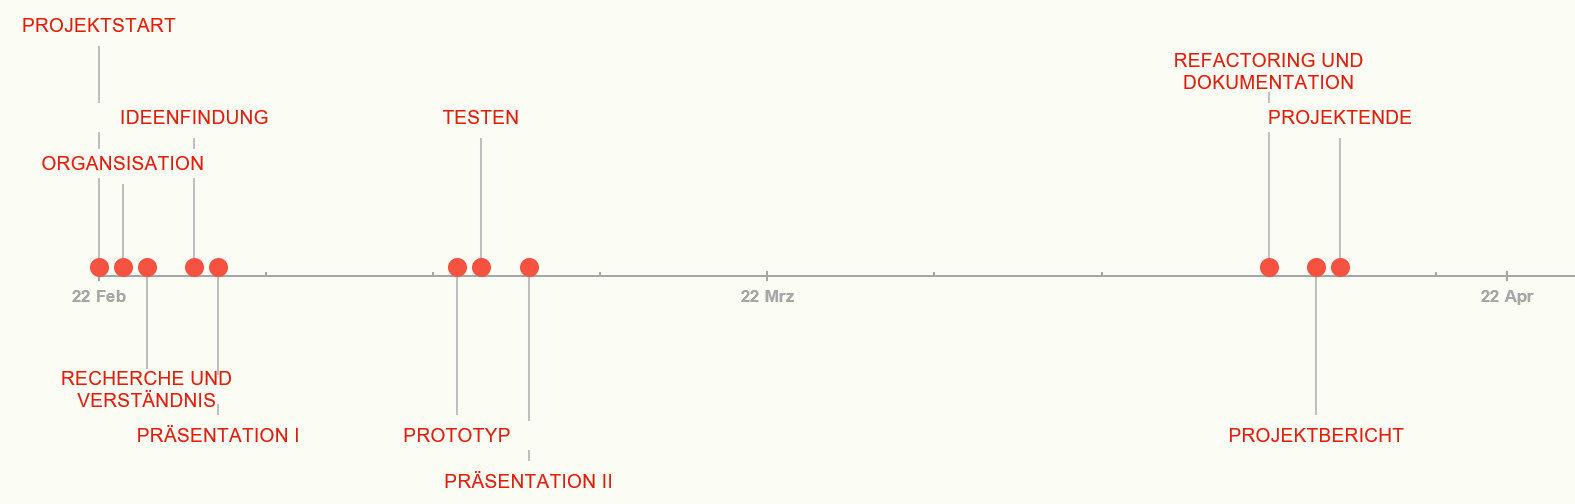
\includegraphics[scale=.5]{meilensteinplan.png}  
\end{center}

\bigbreak
The project started on February 22nd. After a short introduction to the topics and to the Big Data tools like Apache Hadoop, it was part of the agenda to get to know the fellow students and the requirements in general.\\\\
The following day, February 23rd, was primarily used for organization. After a short presentation of the topics on the previous day, the teams were put together and divided into groups of three to four and the topics were narrowed down further. In total, there are two broad topic blocks. Our group decided on the topic block "Social Media Analysis" and chose to conduct a sentiment analysis based on Tweets about COVID-19 in Germany.
After the organizational boundary conditions had been agreed upon, the period from February 23rd to February 27th was intended to familiarize ourselves with the topic. For this purpose, the run time environment was set up and the handling of the provided tools was learned. Helpful was in particular the provided work to the Hadoop literature and the work of Timo Dotzauer and Tobias Lütticke \cite{dotzauer2006}. Through this, the handling of SSH could be comprehended in its effect in addition to the commands provided by the base.camp.\\

After the familiarization research and testing with some samples, the next step was to observe which tools are most suitable for our deployment. Since the relevant tools exhibited a varying degree of maturity we first had to make a suitable selection here in order to be able to define our viewpoint in the next step. Through the previous research and the selection of suitable tools, a suitable choice of ideas could now be made as to how the topic should be implemented in concrete terms. After this was done, it was time for implementation.  \\

Since the project was limited in time, the workload per day was increased accordingly. Since not everything always goes according to plan, a lot of time was planned for plenary discussions and joint bug fixing. Testing always played a role during implementation and was carried out in smaller increments per implementation step. For the final testing of the entire software, therefore, somewhat less time could be taken up, so that this was scheduled with only twelve hours. After the implementation is running correctly so far, the project report is the final step from March 12th. Besides the project report there is also some buffer left to do further bug fixes or improvements of the software.

\section{Daily Meetings}
To ensure that everyone was working towards the same goal and the goal itself was set right, we had 30-minute meetings every day with our mentor, Eugen Rupert. During these meetings, we updated him on our doings and talked about possible impediments. If any impediments could be fixed right away, we would fix them during this meeting. Otherwise, we would schedule follow-ups.

\section{Project management and version control with GitHub}

To grant a continuous workflow over several remote systems, we decided to use the version control and source code management functions of \href{https://github.com/Covidioten}{GitHub}. Due to its amount and variety of functionalities and tools and because we were all familiar with it, GitHub was used for several tasks:
\begin{itemize}
    \item Organization: We created a new organization on GitHub called \href{https://github.com/Covidioten}{Covidioten} which functions as the main starting point for the management of the implementation.
    \item Roadmap and Milestones: We used GitHub for the creation of \href{https://github.com/Covidioten/UI/milestones}{milestones} which were created via GitHub Issues. The milestones were used as signals for important steps on the route from conceptual designs to the first prototype of our product. 
    \item Agile Project Management: Besides the milestones which represent rather higher-level goals, we have also used GitHub issues to assign smaller operational tasks. All the issues and milestones were organized in the \href{https://github.com/orgs/Covidioten/projects/1}{Sentiment Analysis Kanban Board}.
    \item Within Covidioten we created three main repositories: \href{https://github.com/Covidioten/BAPraktikumSentimentAnalyse}{Sentiment Analysis} (MapReduce, Sentiment Analysis), \href{https://github.com/Covidioten/WebServer}{Webserver} (Backend, Hosting, Database) and \href{https://github.com/Covidioten/UI}{UI} (Frontend, GUI, Data Visualization) 
    \item Hosting: We hosted the frontend on GitHub Pages and the backend on our own server.
    \item Automated workflow and testing: To grant a continuous integration, GitHub Actions provides automated building, testing and deploying of the application. 
    \item Workflow: Throughout the project, we worked according to the Gitflow Workflow \cite{GitflowWF}. 
\end{itemize}

\newpage
\chapter{Project documentation}
\section{Architecture}
To build a suitable and well-documented architecture, we followed a template called "arc42". Following this template, we first had to define the constraints and then choose the technology accordingly. The biggest constraint was the continuous data flow and the increasing amount of data. Regarding the scalability, we chose a horizontal approach. In doing so we would only scale the necessary services while the workload is increased and scale them down afterwards. Therefore the costs would be minimal in an idle state. Since this was the only important constraint, we soon started choosing the technologies. To make the horizontal scaling easier, we chose to containerize the backend and the database. A lightweight backend  framework was enough for our purposes and we had Python knowledge in our Team, we chose Flask. In order to store data, we first studied the output of the analyzed data. The data size was reduced from 900GB to only 5Mb. We decided, that big database engine was overhead, we did not need, so we went with SQLite. A user should not only be able to access the data via our backend REST API, but also using a GUI built on Vue.js. Regarding the deployment process, we relied on GitHub Actions and stored our images in the package manager of GitHub.

\begin{figure}[h]
    \centering
    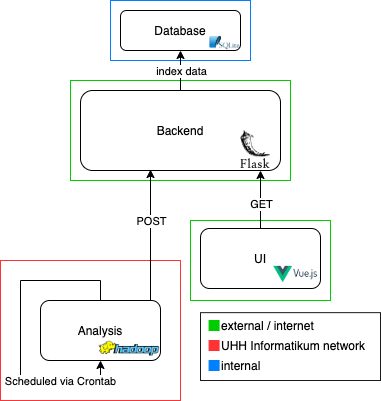
\includegraphics[width=0.75\textwidth]{ArchitectureEng.png}
    \caption{Architecture}
\end{figure}

\newpage

\subsection{Whitebox System}
The system consists of four main parts: data aggregation, data preparation, data analysis, and data publication. The data aggregation and publication is done by our backend and ui, while the our analysis algorithm handled the data analysis. 

\subsubsection*{Data aggregation}
We had to different types of data tweets and political decisions. While the tweets were provided to us by a dataset containing 900Gb of tweets between the 4th of January 2020 and the 31st of December 2020 in a conveniently formatted JSON file, the political statements had to be scrapped. The scrapper is a python script, that is called regularly by crontab.

\subsubsection*{Data preparation}
Since the tweets were well-formatted and cleaned up, we did not have to take any steps regarding the preparation. On the contrary, the scrapped political statements had a lot of mismatches. In our data preparation we reduced the scrapped data to the relevant portions.

\subsubsection*{Data analysis}
Since we had many tweets, we had to process them efficiently. Therefore we iterated over the dataset line by line and used supplementary functions of Hadoop. Further details can be found in the Analysis section.

\subsubsection*{Data publication}
To make the aggregated and analyzed data publicly available, we have implemented an API following the OpenAPI Specification.

\subsubsection*{Interfaces}
The Sentiment analysis produces a JSON File containing the tweets and their sentiment score. To make this data available over the API, we have created a script that sends the file to our webserver to import it there. This script is executed daily by crontab.
The scrapper produces a similar artifact directly on the web server, and the data gets persisted daily.

\newpage

\subsection{Development / Deployment}
Since we used GitHub as our git server and package registry, we have also used it as our CI/CD tool. When adding a commit to the main branch, we test the entire application and deploy it automatically. The backend is being deployed to one of our servers, and the UI is hosted via GitHub Pages. Locally we used a pre-commit hook to lint the respective project. 

\begin{figure}[h]
    \centering
    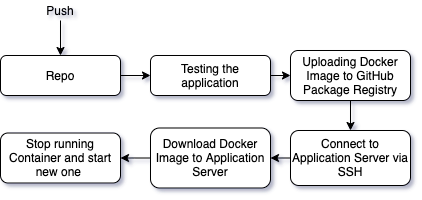
\includegraphics[width=0.75\textwidth]{Deployment.png}
    \caption{Deployment}
\end{figure}

\section{Technical Realization}
One of the core skills that this practical assessment was meant to deliver is to learn how to deal with a huge amount of data effectively. This part of the report will attend to the technical aspects we had to deal with. Its purpose is to give an insight into the circumstances, learnings as well as the problems we faced and how we solved them during the project. 


\subsection*{Python vs Java}
In the beginning we had to make the decision to either use Java or Python to implement the mapper and reducer scripts in. For various reasons we decided on Python. On the one hand Python is a popular choice for data analysis and so we could potentially utilize a great number of frameworks and libraries which help us in our endeavor. This also means that it would be well suited for future plans of adding functionality. On the other hand, the team felt comfortable enough to work with python other than Java. 

\subsection{Data}


\begin{figure}[h]
    \centering
    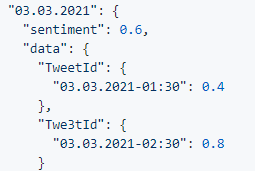
\includegraphics[]{data_structure.png}
    \caption{Example of how our data looks like}
    % \label{fig:my_label}
\end{figure}

The data we used was already provided for us so, even though it would have been an interesting part to learn, there was no necessity to figure out how to import it and for simplicity we decided to focus on our main objective, so we did not use our own data. The data consists of about 900 Gigabyte of Twitter Data which dates from 04.01.2020 to the 31.12.2020. The provided data was conveniently formatted in JSON line. This had two huge implications for us. First of all, we did not need to do any tedious data cleaning and structuring of the data on our own. The second advantage is that because the dataset is so big, it would be impossible to load a huge JSON object at once. So having a line represented by a JSON object for a single post makes it perfect to iterate over and load each JSON object separately. For every Tweet JSON object that we got we had a variety of key- value pairs related to that tweet. However, because we only needed a few information most of it was not considered. For us the interesting values were in the keys “text” – containing the actual Tweet Text to calculate the sentiment from, “created\_at” -  which held the date at which the Tweet was created. We also took the Tweet ID from the “id” key to use as an identifier for our own data. This also had the advantage that we could easily test if our data was created correctly. 

\subsection{Hadoop}

Hadoop is a framework to manage and process large amounts of data on several distributed nodes. Its distributed nature allows for computation in parallel. It also implements configurable functions to ensure redundancy in case of partial failure.

To get started with Hadoop we had a video lecture from our mentor Eugen Ruppert, explaining the basics of Hadoop. There were two main components to get familiar with. The CLI part and the Dashboard for status and debugging. Hadoop is mainly operated through a CLI, so brushing up some of the Linux Terminal skills was necessary to effectively navigate the Hadoop functions as well as learning a few new Hadoop related commands. For debugging purposes, we had to connect to the web dashboard of Hadoop and see the log files. 
\begin{center}
\begin{figure}
    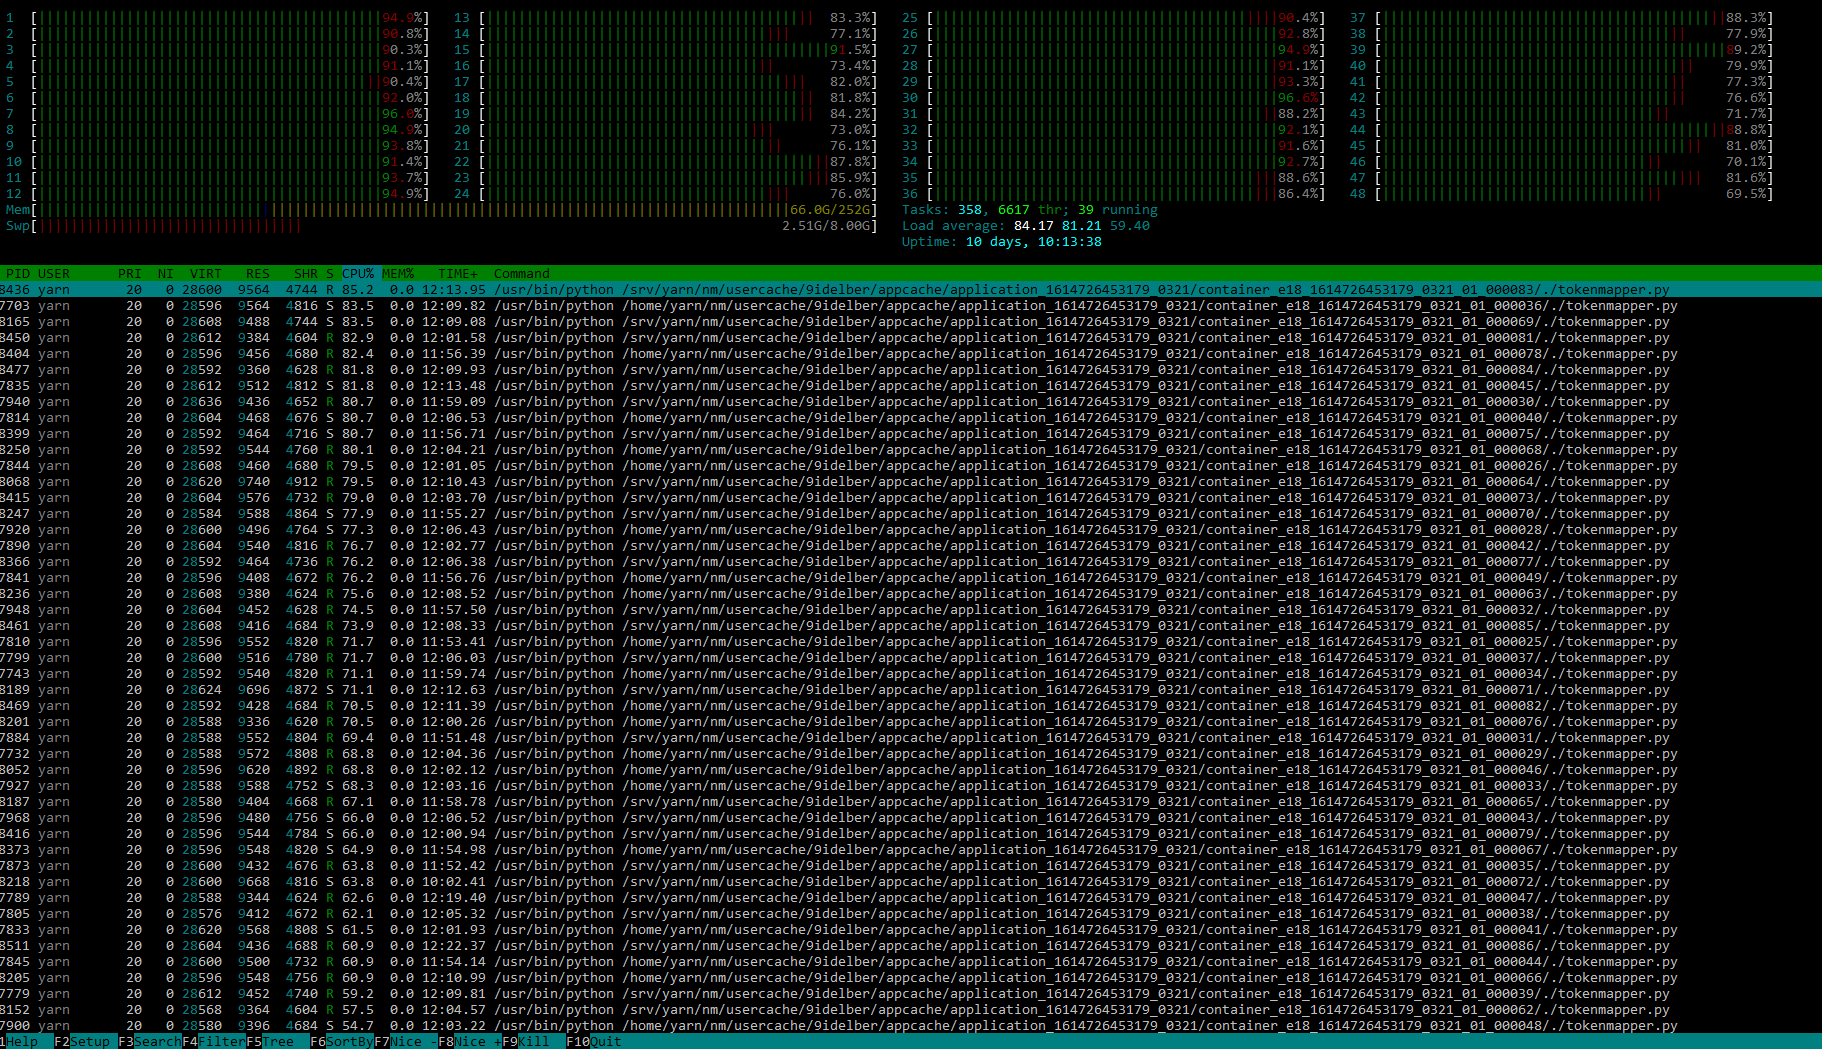
\includegraphics[scale=.35]{cluster.png}
    \caption{The 'Informatikum' Cluster while running a map/reduce job}
\end{figure}
\end{center}


\subsection{MapReduce}
To analyze our data, we used a two staged process called mapping and reducing. This is a process which can utilize the distributed nature of the data stored. The mapping is basically assigning a specific value to each entry of the data. To do this effectively every node in the cluster can do this independently in parallel. Once every data entry has been labeled with a value, it gets reorganized internally so that data entries with the same value get to be grouped together. In our case we extracted the date of the Tweet and printed a “1” to count the total posts per day. This concludes the mapping stage of the process. In the reducing stage we iterate over the mapped and grouped elements. Whenever an entry that deviates from the entry before occurs we know that the entry before the new entry was the last one because the elements are grouped. So we can give a total output as the sum of all values for that entry. In our case we generated a JSON file containing the total amount of tweets per day and the amount of tweets that had a sentiment score that is not 0, the average sentiment for the day and the tweets represented by its id. Tweets consist of the time of its creation and the sentiment score.


\subsection{Sentiment Analysis}

\subsection*{What is sentiment analysis?}

Sentiment analysis is the process of automatically evaluating the sentiment of a text. Its goal is to detect the intensity of the positivity or negativity within that text.


\subsection*{How sentiment analysis works}
There are several possible procedures to determine a sentiment for a given text. One the most efficient and popular methods to detect a sentiment is to train an artificial neural network to recognize patterns of speech associated with positive and negative meanings. Without going into too much detail, we shortly want to give an idea of how the general structure of such an approach would work. First a labeled dataset of texts that are comparable to the ones you want to determine a sentiment from is created. Then the neural network gets trained on the dataset. After training the network is tested on a test dataset that the neural network has not been trained with to measure its performance. If the performance is sufficient the neural network can be used to analyze the data you want to get a sentiment from. To simplify the process of training a model there exist frameworks such as “spaCy” to assist you in doing so. However it is still a time consuming process and we could not find a reliable German dataset to train a model on. However for future updates it would be an interesting feature to look into.

\textbf{Conclusion:}
\begin{itemize}
    \item Advanced technique
    \item More accurate sentiment estimation
    \item Time consuming process
\end{itemize}

\textbf{Problems:}
\begin{itemize}
    \item Artificial neural networks naturally do not behave deterministically
    \item Is prone to subjectivity
\end{itemize}

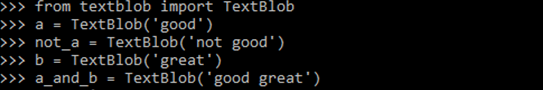
\includegraphics[]{basic_usage.png}

In order to stay on track with our timeline we decided to use a simpler way to get into the field of sentiment analysis.
A very basic technique is to compare every word of a text to list of words that has been pre-labeled with a specific sentiment value. Words that have several meanings have different sentiment values for each meaning. So what Frameworks like TextBlob do is they just average over all the different sentiment values. \\

\begin{center}
    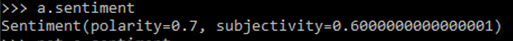
\includegraphics[]{a.png}\\
    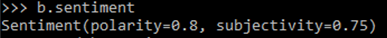
\includegraphics[]{b.png}
\end{center}

Obviously this is a drastic simplification and therefor is not extremely accurate, but it allows for a naive sentiment analysis. Negations are handled by just multiplying – 0,5 to the value of the word that the negation refers to.\\

\begin{center}
    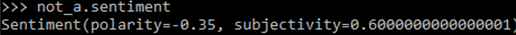
\includegraphics[]{not_a.png}
\end{center}

If the text provided to the TextBlob contains a variety of words with a sentiment value TextBlob will take the average of all sentiment values. 

\begin{center}
    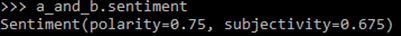
\includegraphics[]{a_and_b.png}
\end{center}
 
\textbf{Conclusion:}

\begin{itemize}
    \item Easy to use
    \item Out of the box solution
    \item Good starting point to get familiar with sentiment analysis
    \item can be unreliable
\end{itemize}

\textbf{Problems}

\begin{itemize}
    \item Makes drastic simplifications
    \item Doesn’t consider the context (sarcasm etc.)
    \item Is prone to subjectivity
\end{itemize}

\subsection{Challenges}
Twitter is a service used from all around the world. However datasets usually only work for a specific language. To compensate this fact we concentrated on German support for our MVP. To get a more global impression more languages could be added in the future. We also had an issue with the encoding of the tweet text which worked in the test cases with little data, however running on the cluster it was giving us an error we did not know how to interpret so we had to get a little help from our Mentor. We also realized how important it is to coordinate the resources of the cluster because there can occur situations where you compete between them. 

\section{Backend}
To build a scalable and performant backend, one of the most important aspects is the data structure. Therefore we have designed an entity-relationship diagram and created a database scheme accordingly. Since a lightweight solution was enough for our purposes, we chose Flask as our backend framework and connected it to an SQLite database.

\subsection{ER diagram}
Our system consists of two entities. The first one is the sentiment itself, we have called this one a "DataPoint," and the political statements, which we have called "News". A DataPoint represents an entire month. We only save a "News" entry per day and therefore have a One-To-One relationship. Since our UI presents the data grouped by month, we did not create any further objects for the daily sentiments or tweet sentiments themselves.

\begin{figure}[h]
    \centering
    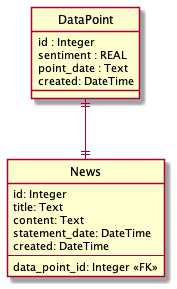
\includegraphics[]{ER-Diagram.png}
    \caption{ER Diagram}
    % \label{fig:my_label}
\end{figure}

\subsection{Technologies}
When implementing the functionality, we thought about the tooling, libraries, and concepts to help us during the development. We decided to create our diagrams using PlantUML, created an OpenAPI specification, added pytest for testing purposes, black for code formatting, and finally created an SQLite database to store the data. Flask itself comes with many features, so we did not need to add a significant amount of dependencies.

\subsection{Packaging and Deployment}
We install the necessary dependencies on every push to the main branch, test the application, build a docker image, and push the image to the GitHub package registry. From there on, the deployment to one of our servers started.

\subsection{Outlook}
To further improve the application, two important features should be implemented / added. 
The first one would be to restrict certain routes, to prevent anonymous users from inserting invalid data into our database.
The second one would be to improve the code quality by adding static code analysis and a quality gate to the deployment process.

\section{Frontend and data visualization}

\subsection{User-centered design and implementation of the frontend}
Before the actual implementation of the frontend, important questions regarding the context of use had to be clarified. In doing so, we followed a user-centered design process (UCDP). The UCDP is an iterative process that focuses on the requirements, goals, and characteristics of the users during development \cite{abras2004user}:

\begin{figure}[h]
    \centering
    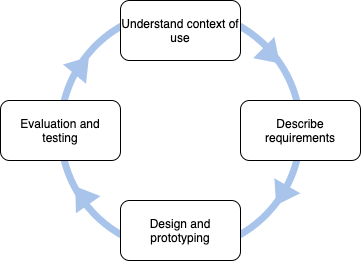
\includegraphics[width=0.5\textwidth]{pic/UCDP_English.png}
    \caption{User centered design process \cite{norman2013}}
    \label{fig:my_label}
\end{figure}

\begin{itemize}
    \item \textbf{Context analysis}: The users come from any age group from 1 to 99 and have an interest in current developments of the COVID-19 pandemic in Germany. The aim of the users is to analyze the sentiment of the German population. At the moment, the analysis is retrospective to the year 2020, but could be extended to real-time data.
    \item  
    \textbf{Requirement analysis}: Users should be able to read off the most important information quickly and in an easily recognizable way so that they can quickly answer their questions regarding the sentiment in the German population. To achieve this goal, we decided to prepare the information graphically and visualize it as a chart (see Data Visualization). \\
    In addition, we would like to show a quickly recognizable connection between Twitter sentiment, COVID-19 case numbers and political measures in Germany. For this, we need features that clearly link all three metrics. \\
    In addition, users should be able to understand how the data was collected and which sources were used. Furthermore, it should be explained what sentiment is, how the sentiment analysis was conducted and what the goal of the web application is. \\
    This serves to ensure that the data is presented as transparently and credibly as possible. In addition, users should be informed about the analysis in order to gain as much insight as possible from the application and to eliminate possible ambiguities. 

    \item \textbf{Design and prototyping}: In order to obtain initial user feedback as early as possible, it is advisable to work with wireframes and prototypes of the graphical user interface (GUI) in order to already gather opinions from potential users and possibly conduct initial tests. In our case, mockups were required for the first plenary presentation.
    
    \item \textbf{Evaluation and testing}: After prototypes have been developed, they are to be tested. As described above, our testing was limited to feedback from the plenum of the base.camp and small thinking aloud tests within the team members. For the further procedure, it suggests itself to carry out thinking aloud or A/B tests with a user sample in the next step.
    
    
\end{itemize}

\subsection{Design and implementation of the graphical user interface (GUI)}
As mentioned above, the GUI needs to fill the users' need to analyze and understand the possible correlation between the sentiment on Twitter and the number of COVID-19 cases in Germany. Therefore, it needs a visualization of the data and an explanation of the data and the term "sentiment".\\
To implement those features, we needed to find the right tools and libraries to draw on pre-built features. \\
First of all, we decided that we want to build a web-app that is mainly used on desktop computers. In the next step, we did research on popular framework and libraries to build web-apps. From React.js, Angular and Vue.js we decided to use Vue.js since it is simple to get started, has a great documentation, strong community support and it is not developed and maintained by some huge corporation like Facebook or Google.\\
For the visualization, we selected \textit{Chart.js, ApexCharts.js and Plotly} as suitable chart libraries. Due to its simplicity, understandable documentation and an easy implementation with Vue.js, we chose ApexCharts.js as the most favorable solution. \\
\\
Because of its component system every feature of a website built with Vue.js is implemented in its own component. Hence, the whole application consists of many smaller components. In our case, we created one component for the chart, the explanation of the sentiment, the info section, the footer, and the imprint. On top of that is a generic vue app component which respectively is initialized by the main.js class. \\

\subsubsection*{Views}
To provide a clear interface without information overload, it is  possible to have only one view at a time. For this implementation we used the official Vue Router technology which makes it possible to create several views and to switch between them on a single-page application. We implemented one router-view in the center of the page. By several buttons above the view, the user can switch between the chart, the sentiment explanation or the info section. In the footer, there is a link to the imprint which is also shown in the mentioned router-view.

\subsubsection*{Chart}
The chart view shows the main data and information. It will be explained in the detail in the chapter \textit{Data Visualization}.


\subsubsection*{Sentiment explanation}
After getting feedback from other participants of the base.camp it was brought to our attention that an explanation of what sentiment actually is was missing in our prototype. Since sentiment is such a central term in our application it is almost unusable if the user does not know what sentiment is. Thus, we created another view which sole purpose is to explain what sentiment means and how to read it. \\
To make it more comprehensible to the user, a rather impatient tweet by Donald Trump and its respective sentiment calculated by TextBlob was added as an example. To the contrary, the phrase "I love university" with a sentiment of 0.5 is shown. 

\begin{figure}
    \centering
    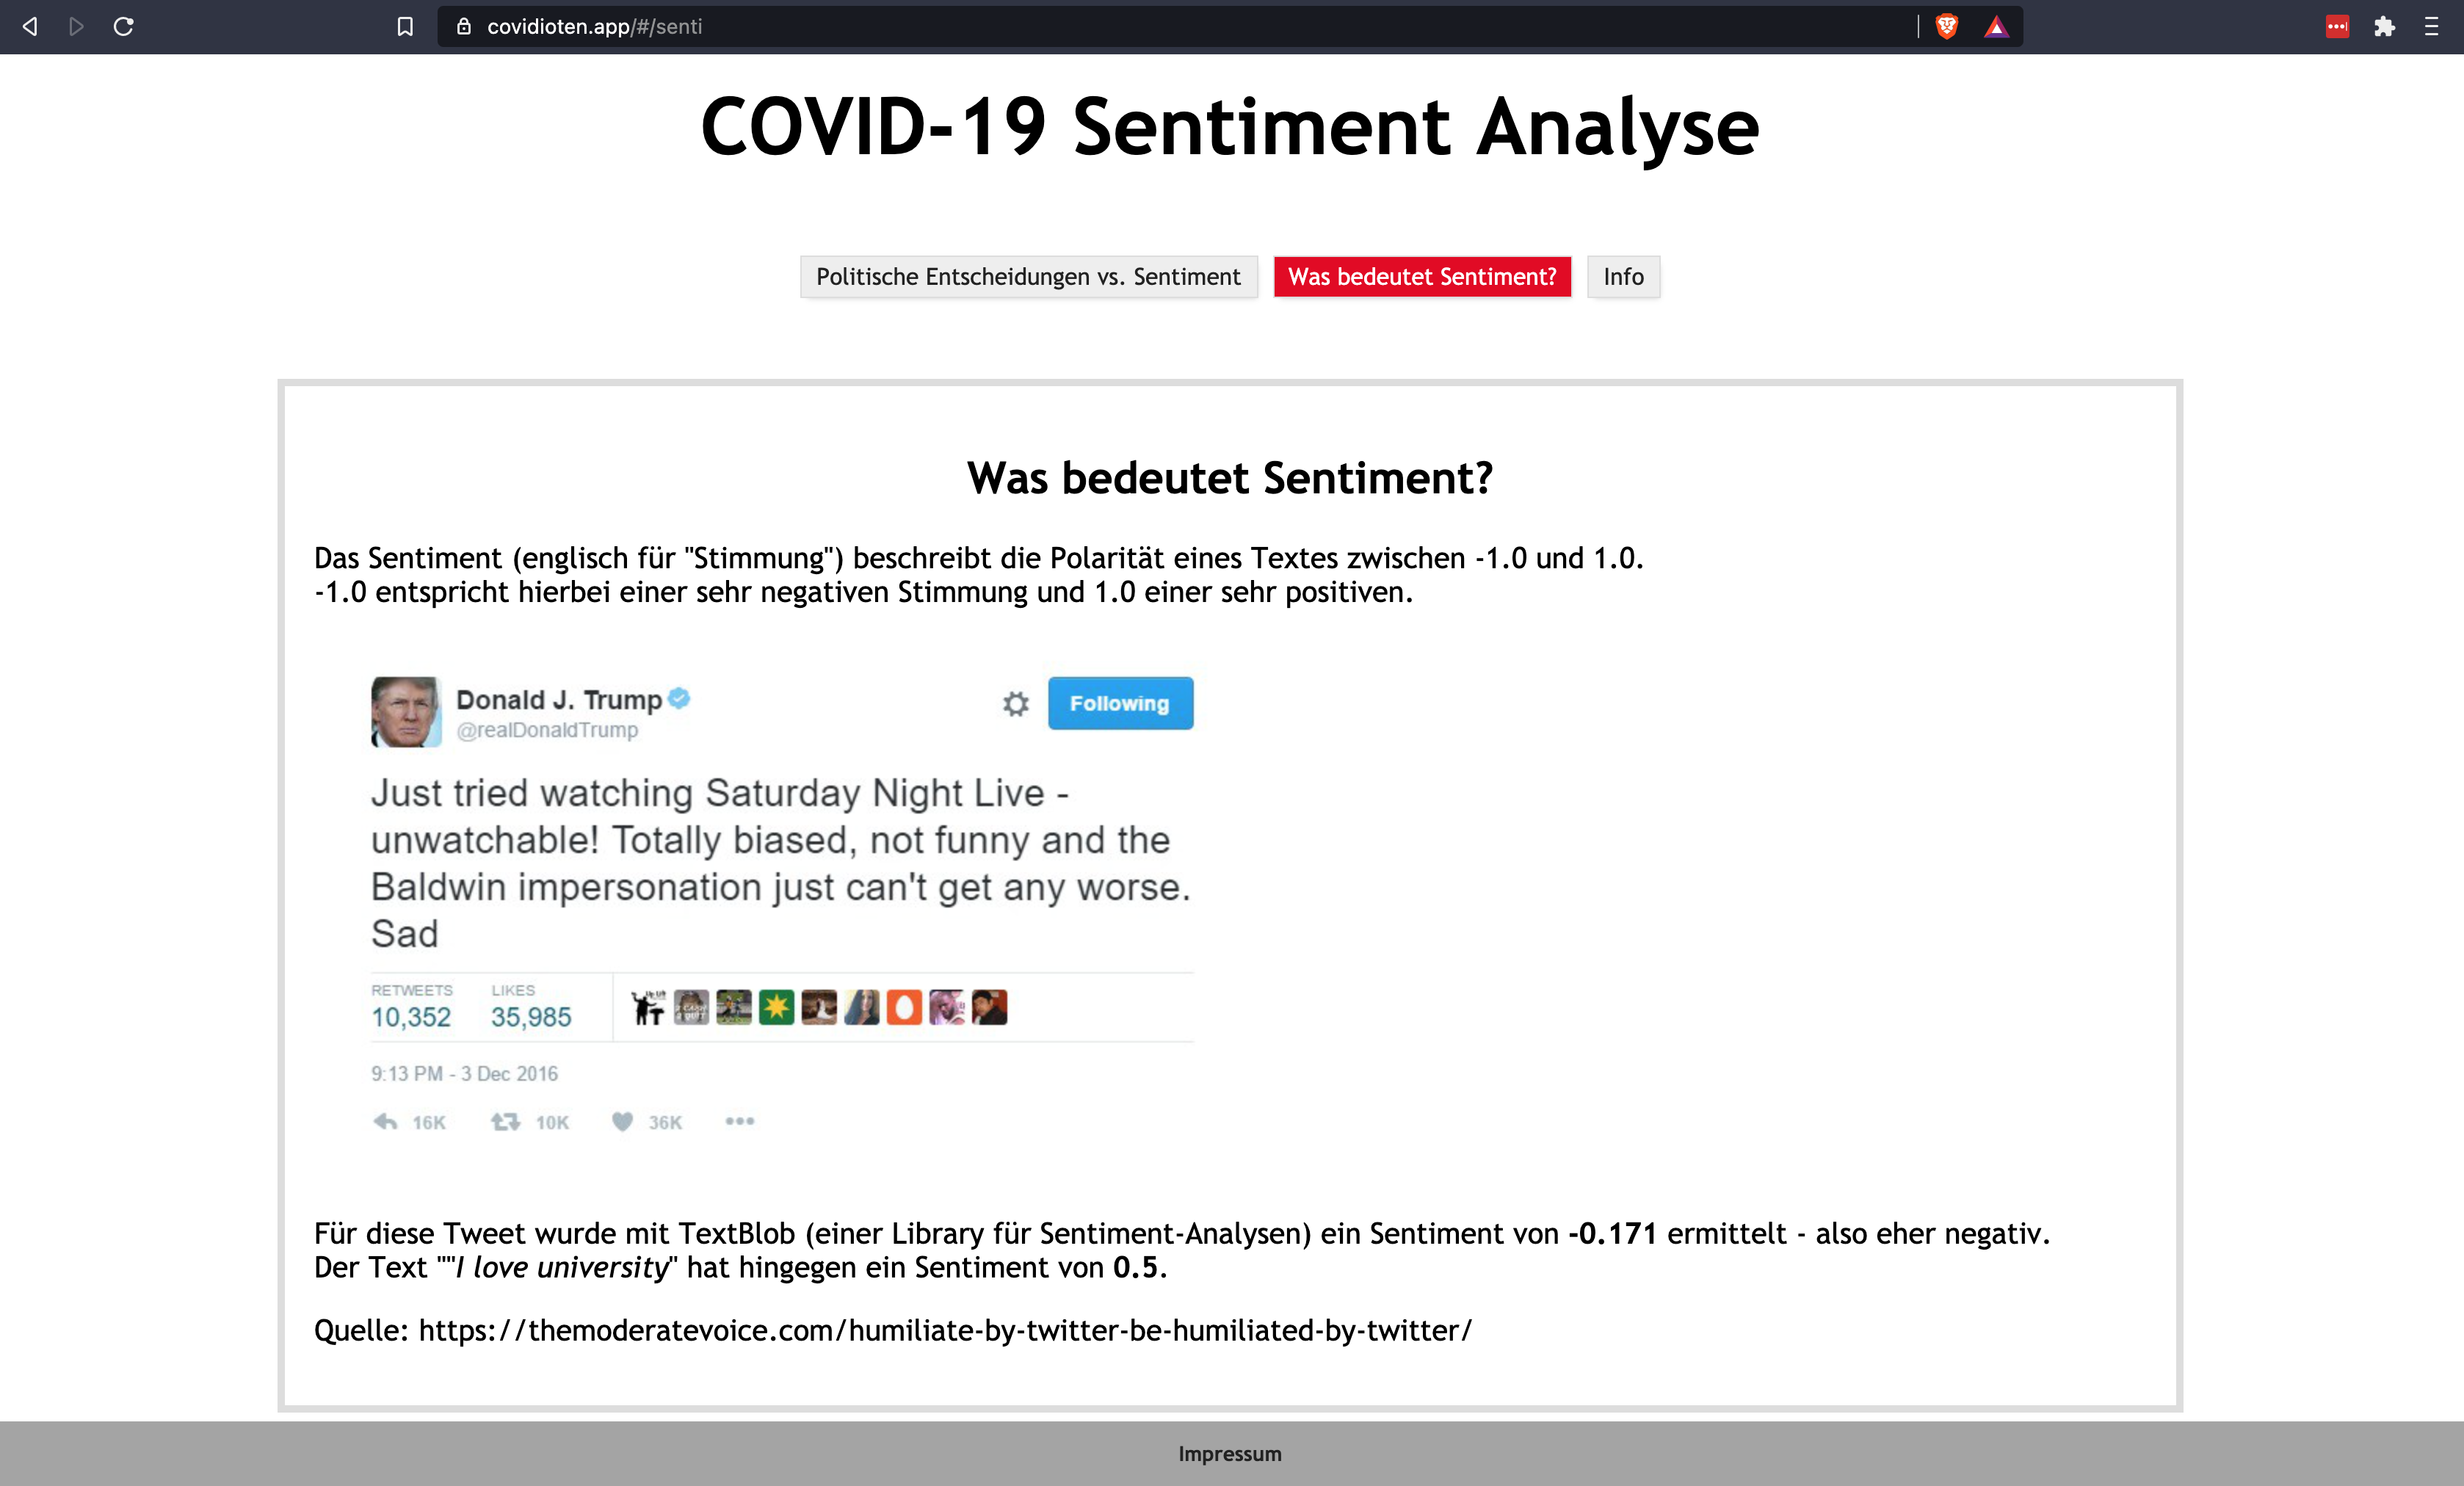
\includegraphics[width=1.0\textwidth]{pic/Senti-Explanation.png}
    \caption{Sentiment-Explanation-View}
    \label{fig:my_label}
\end{figure}

\subsubsection*{Info}
In the info section, the user will find basic information about how the data was collected and what is shown in the chart. Furthermore, it describes the outline of this project and the web application. Hence, the user will understand the objectives of this app and how to use it. Furthermore, to meet academic standards, the sources of the political news sites and the source of the active COVID-19 cases are linked in this view.

\begin{figure}
    \centering
    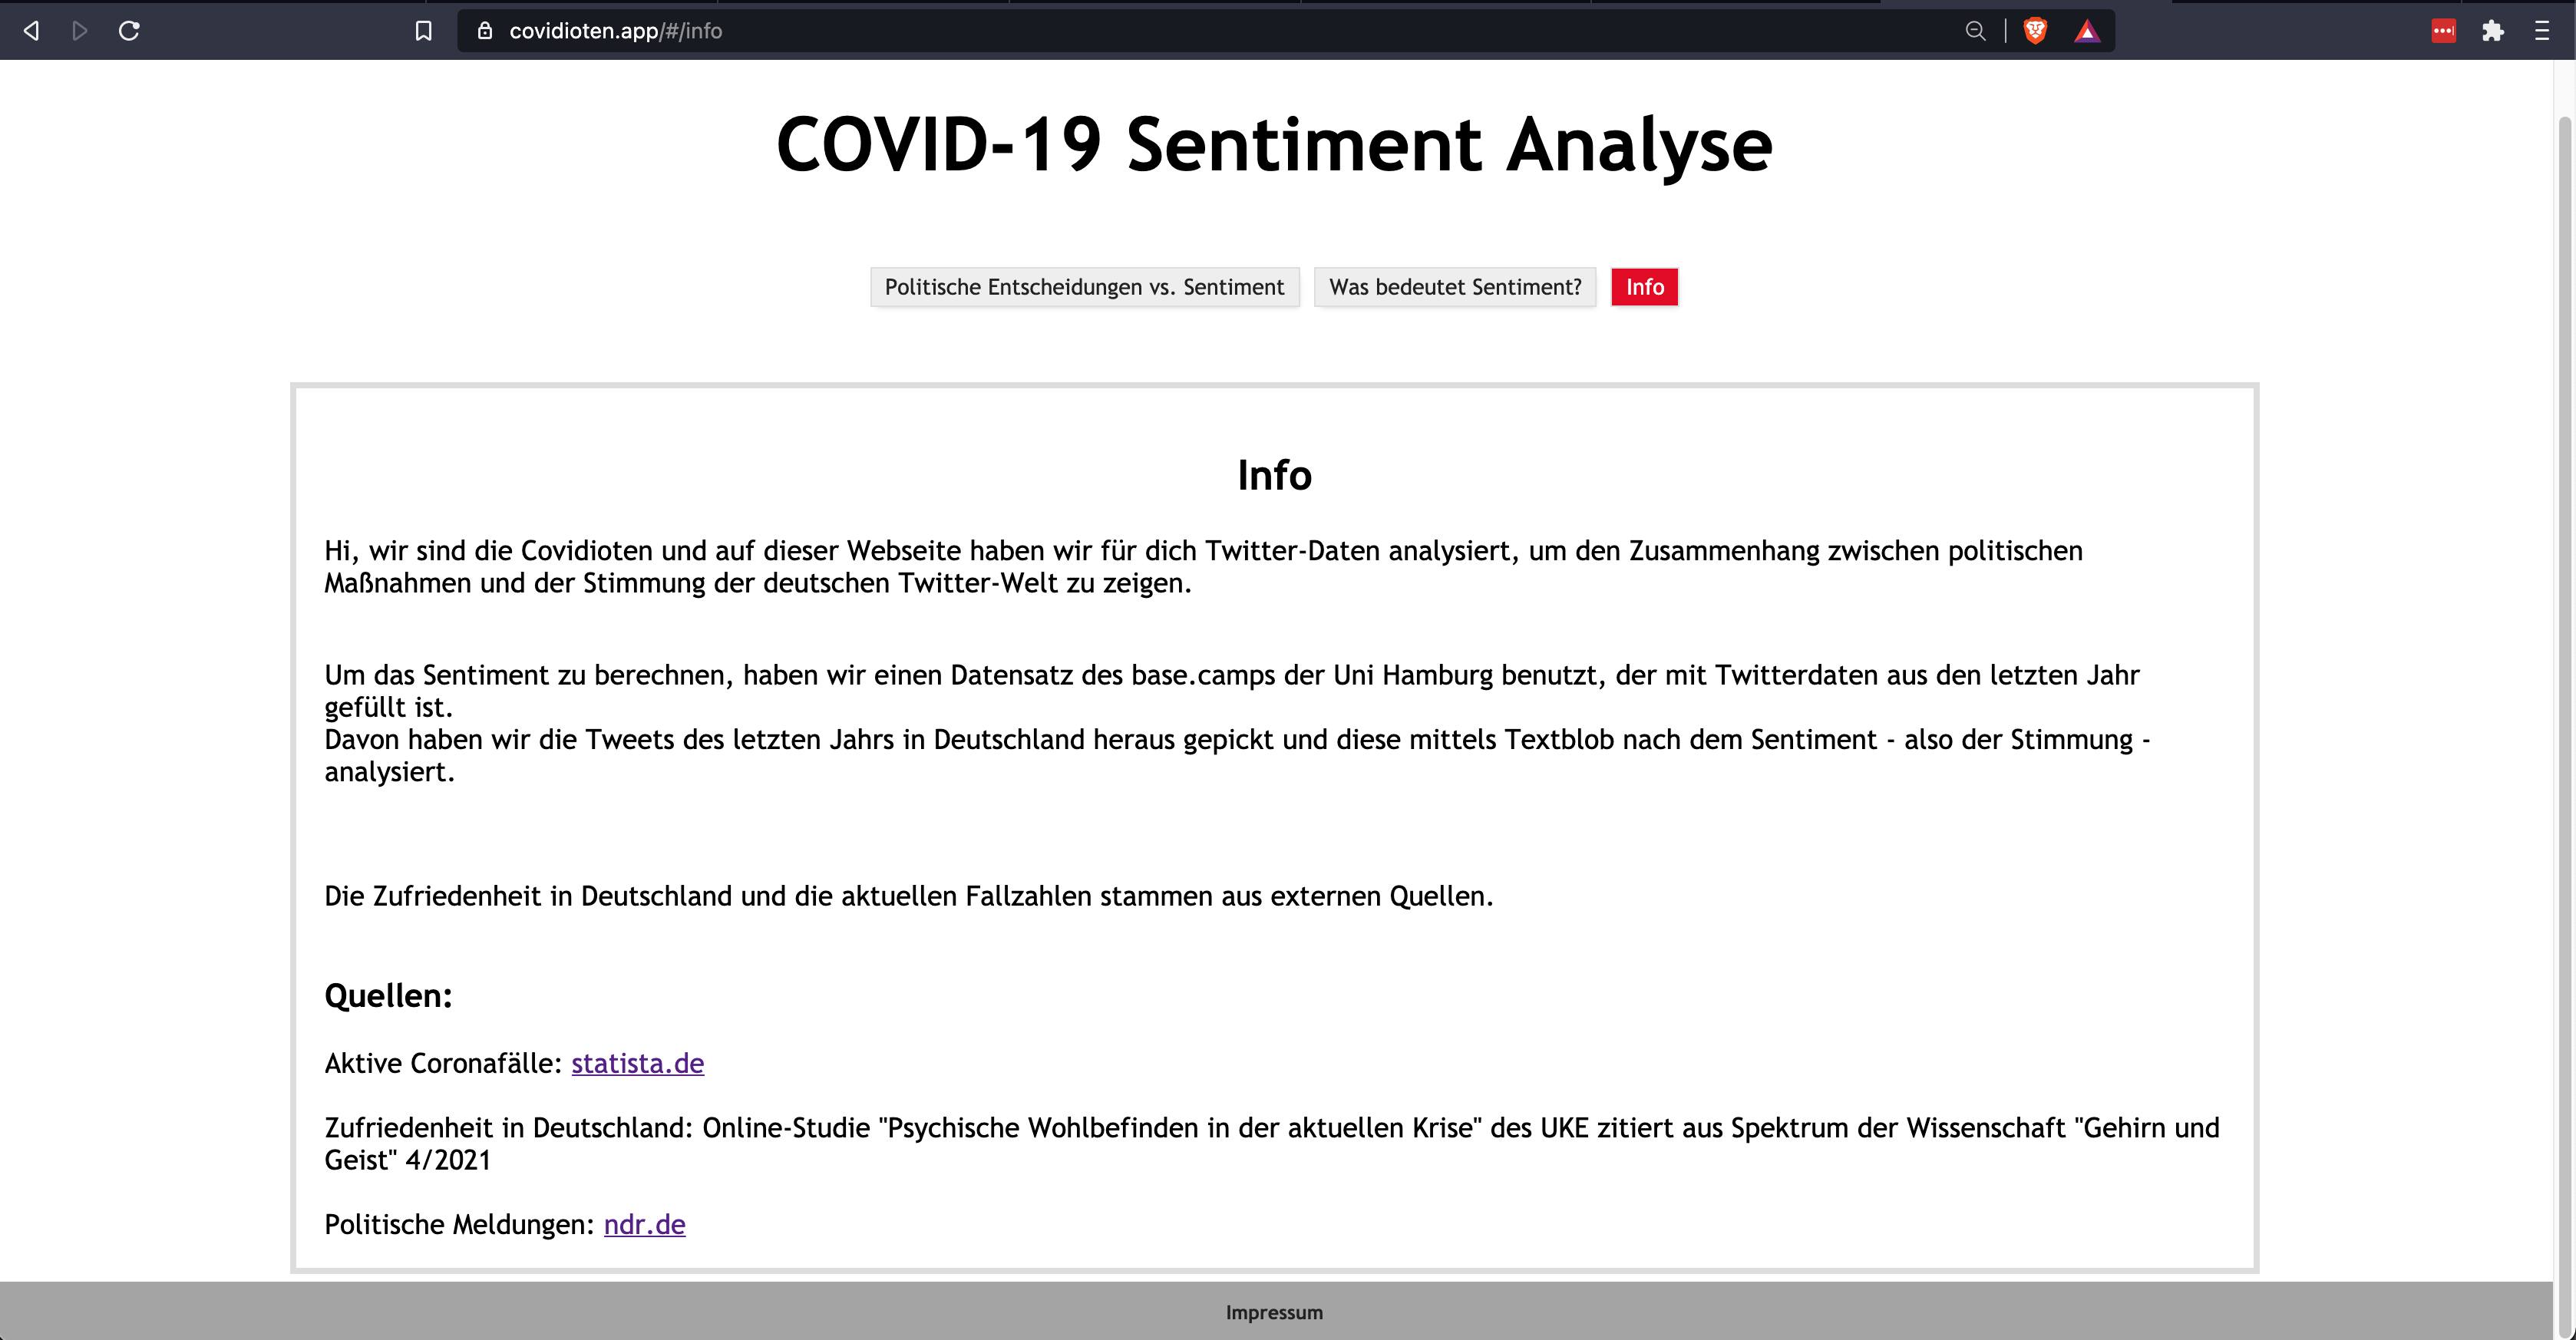
\includegraphics[width=1.0\textwidth]{pic/Info-Section.png}
    \caption{Info-View}
    \label{fig:my_label}
\end{figure}


\subsubsection*{Footer}
The footer bar serves as a solid component on the website and sticks on the bottom edge of the site. It only holds a link to the compulsory imprint. Similar to the buttons above the view, the imprint is linked view "vue-router" and is shown in the router-view container.

\begin{figure}[h]
    \centering
    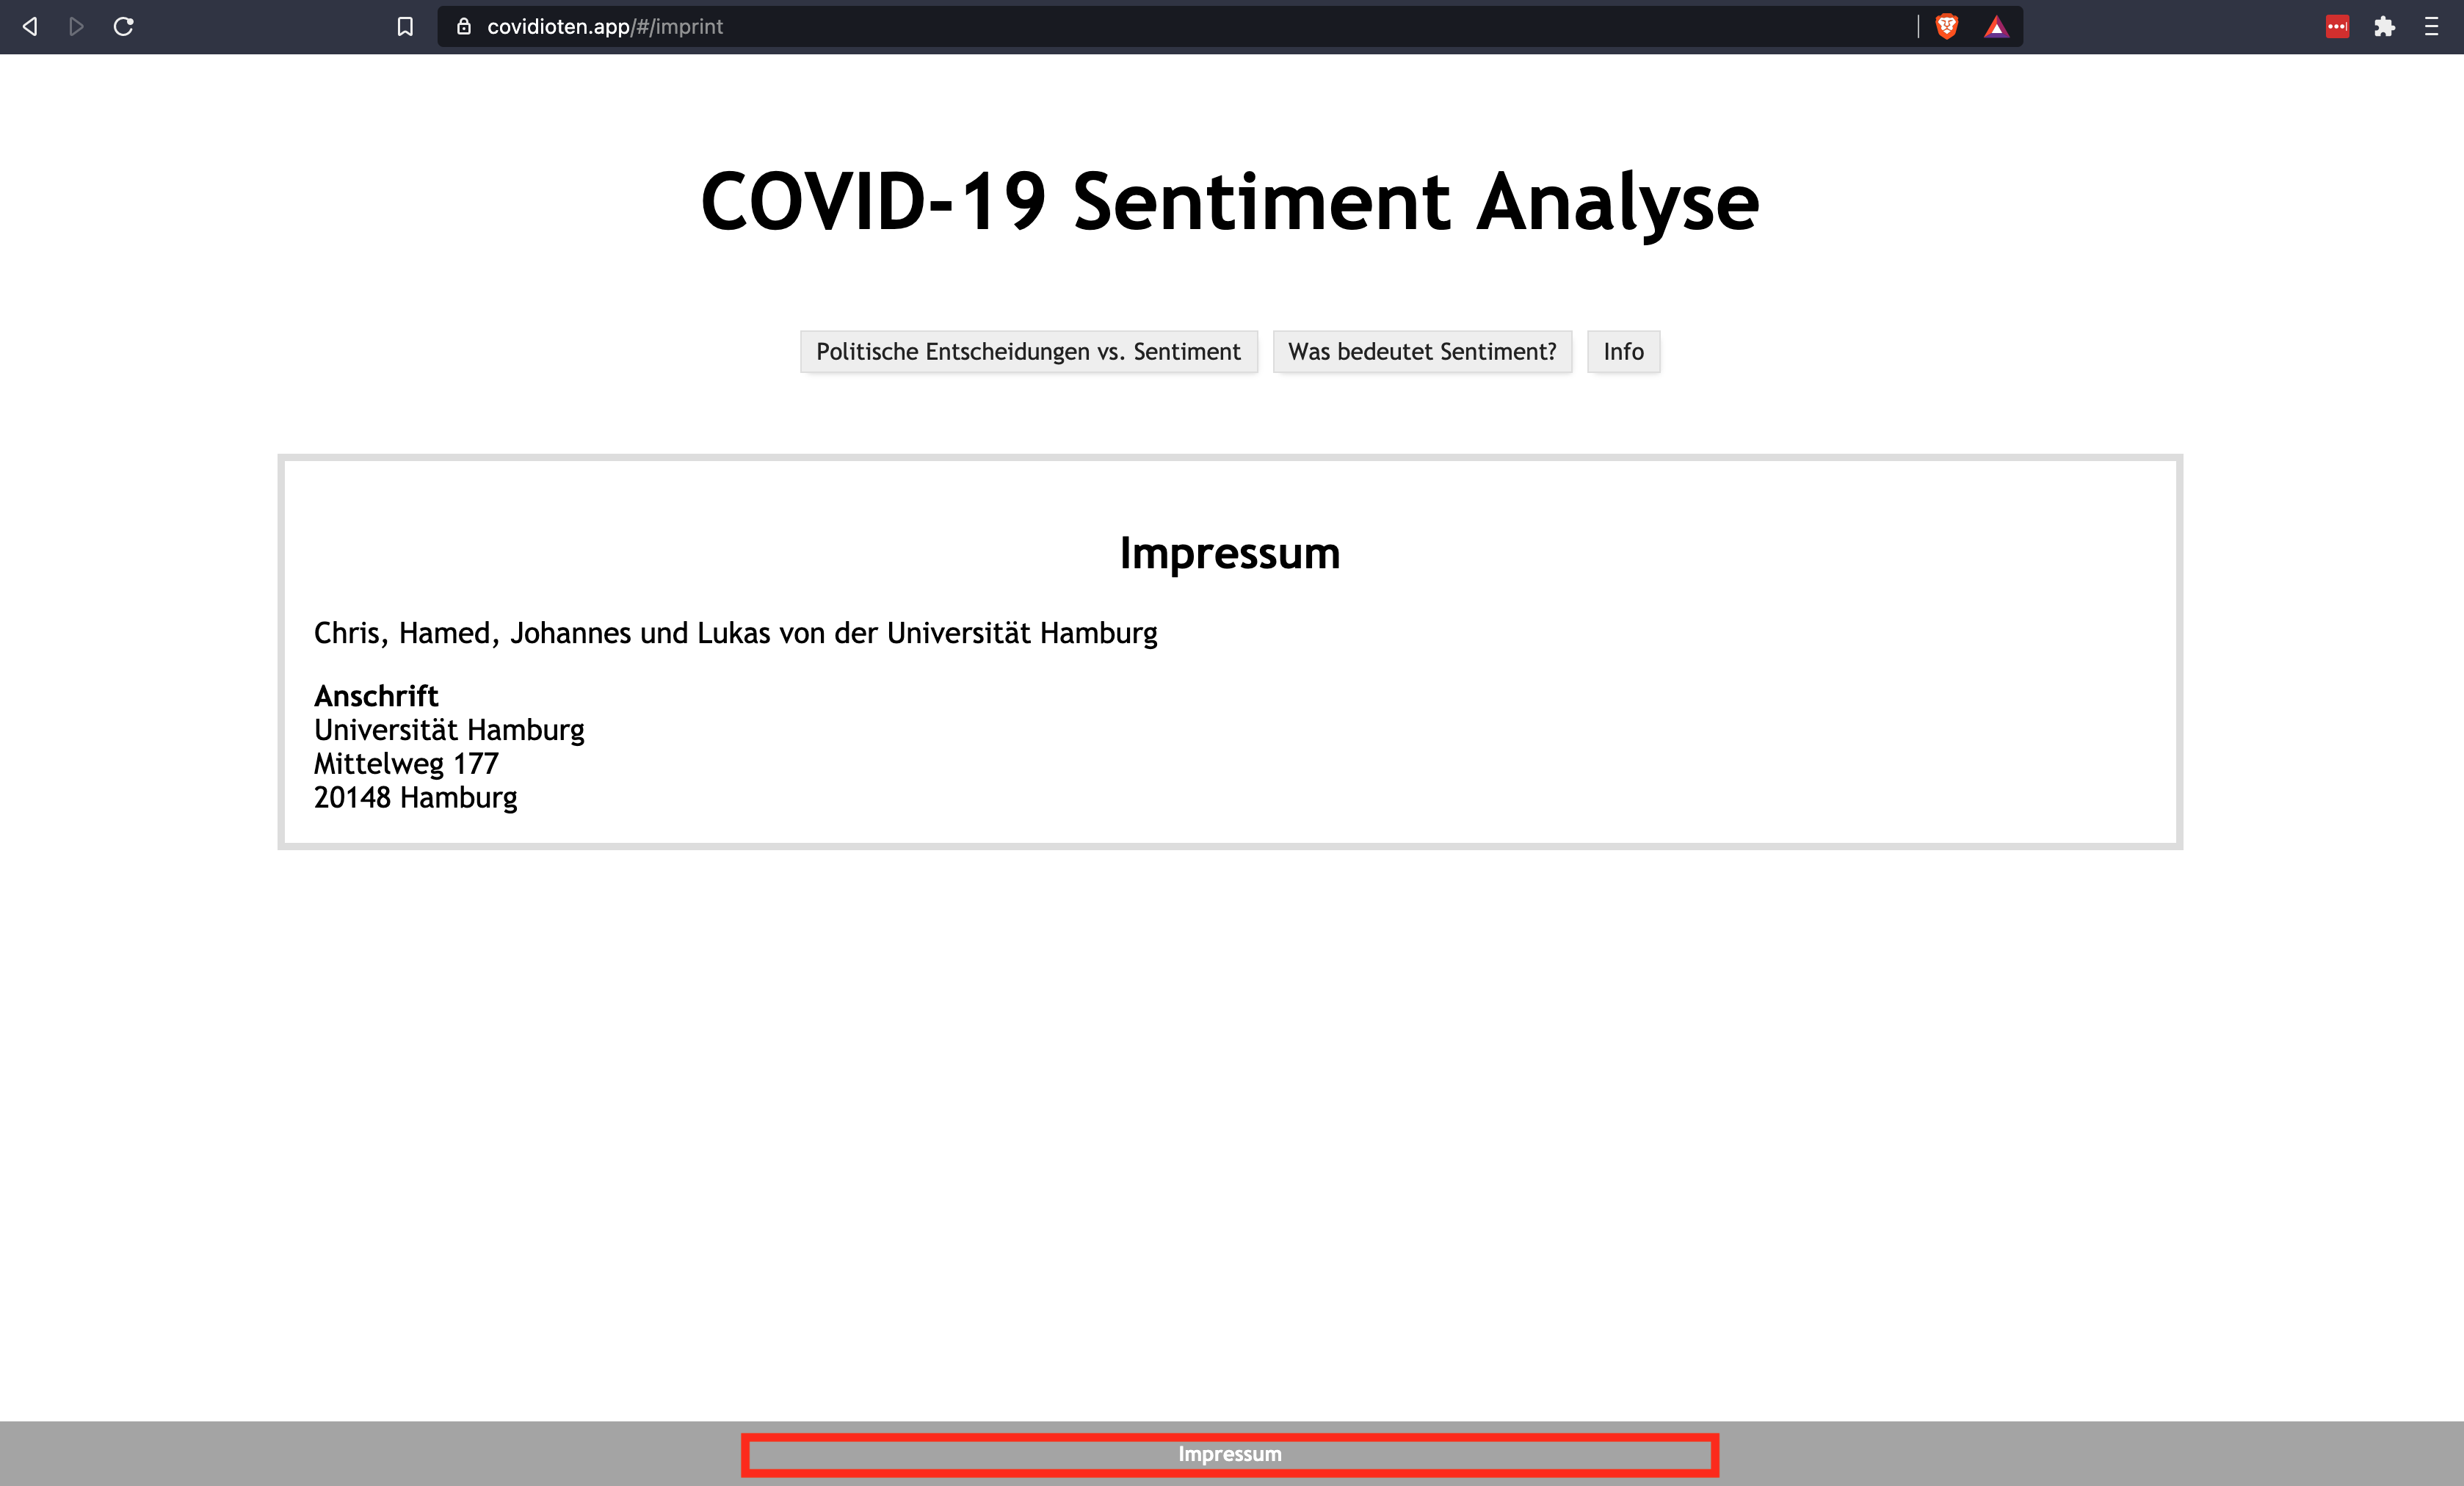
\includegraphics[width=1.0\textwidth]{pic/Imprint.png}
    \caption{Footer and Imprint}
    \label{fig:my_label}
\end{figure}

\subsubsection*{Imprint}
In the imprint view the user can find information about the web masters and the address of the University of Hamburg to get in contact with the creators. 



\subsection{Data Visualization}
As mentioned above the library ApexCharts.js was used to visualize the data we generated through the sentiment analysis. ApexCharts gives us the possibility to choose between several chart types. The objective of our chart was to show a possible correlation between COVID-19 cases in Germany, the average sentiment of German tweets, and political news and measures taken at a specific time in the year 2020. \\
After some brainstorming we decided that the most intuitive way to show the amount of cases is a basic line graph. However, in order to create a strong differentiation between the number of cases and the twitter sentiment, we used a bar graph for the twitter sentiment. \\
The x-axis shows the months of the year 2020 in continuous timely manner. Due to the structure of the analyzed data and for interface simplicity the sentiment data was clustered into monthly averages.\\
Since the twitter sentiment and the COVID-19 cases have fundamentally different scales (sentiment: 0.01 - 0.13 and COVID-19 cases: 0 - 380.000), we used two different scales for each data line. \\
To feature political measures, we created a third data line on top of the twitter sentiment. However, we set the line thickness to zero in order to only show the data points per month. We used the so-called "tooltips" that come with ApexCharts to display information about the political situation in Germany. The tooltips can be customized via plain HTML and CSS implementations and they are only shown when the users hovers over the red data markers. 

\begin{figure}[h]
    \centering
    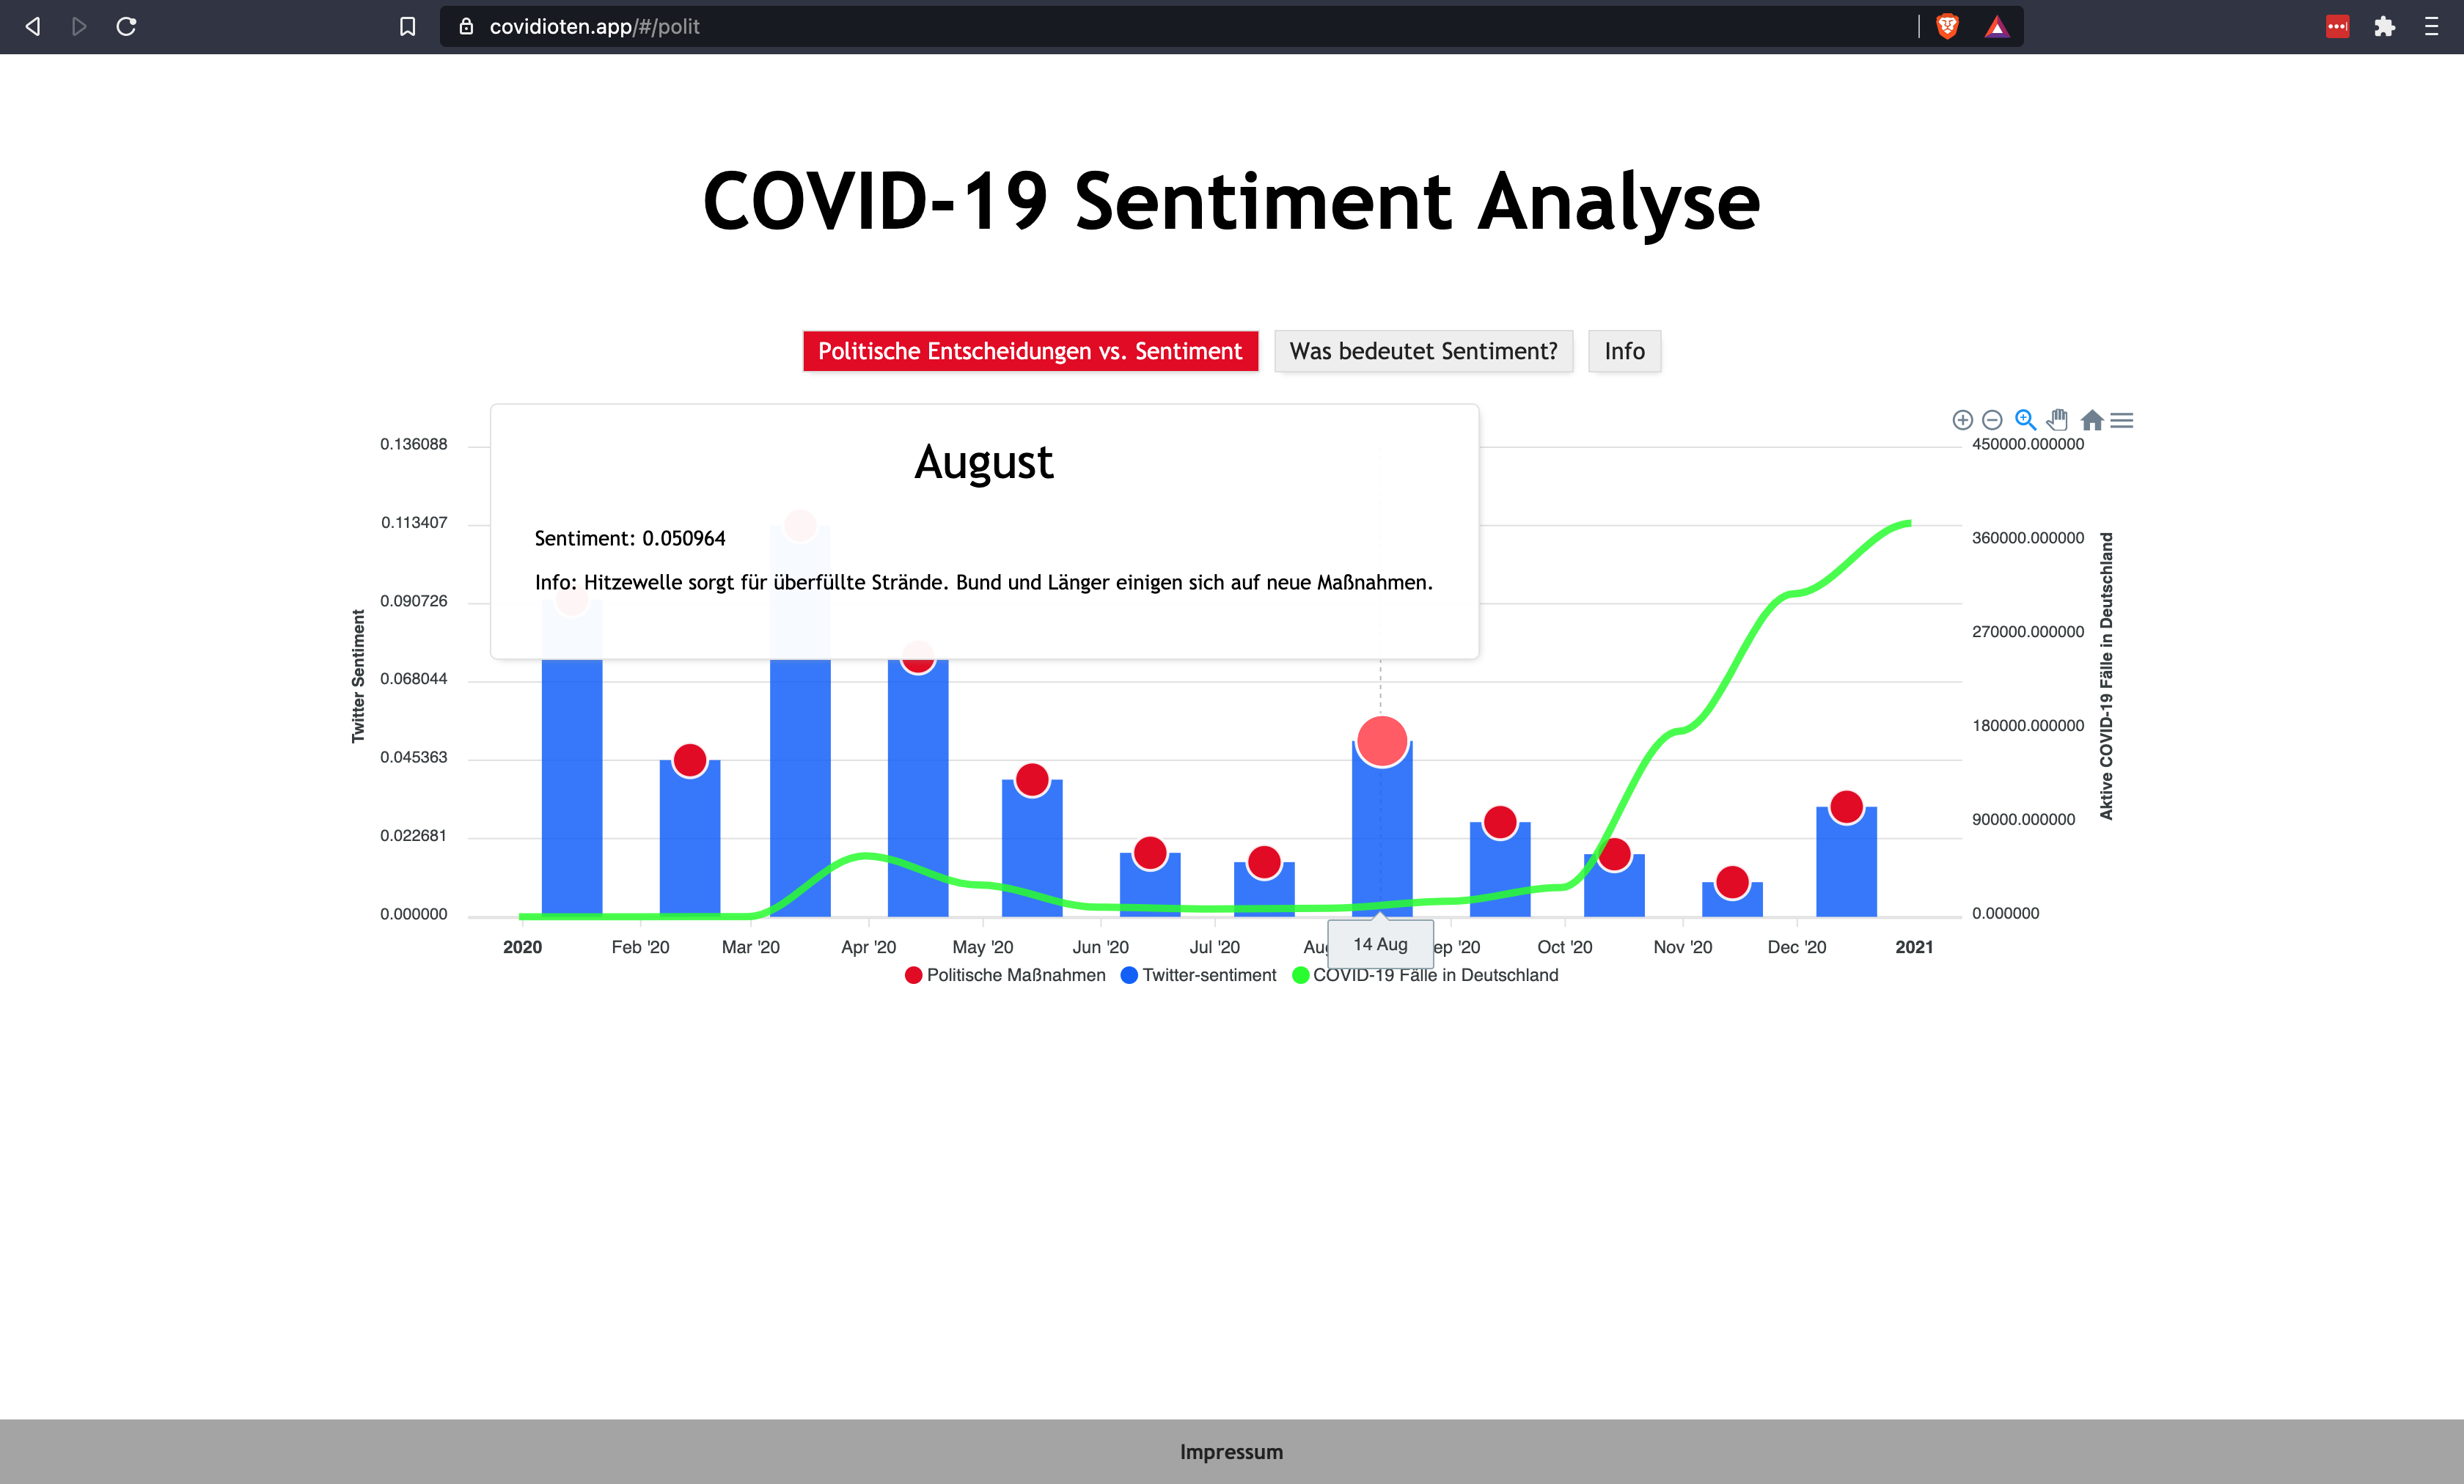
\includegraphics[width=1.0\textwidth]{pic/Tooltips.png}
    \caption{Chart visualization and Tooltip}
    \label{fig:my_label}
\end{figure}

The data for the political situation in Germany was collected from the Northern German Broadcasting NDR \cite{ndr} that published a website with the corona chronology in Germany in 2020.\\
All three data lines can be switched on or off by clicking on the tags above the chart.

\begin{figure}[h]
    \centering
    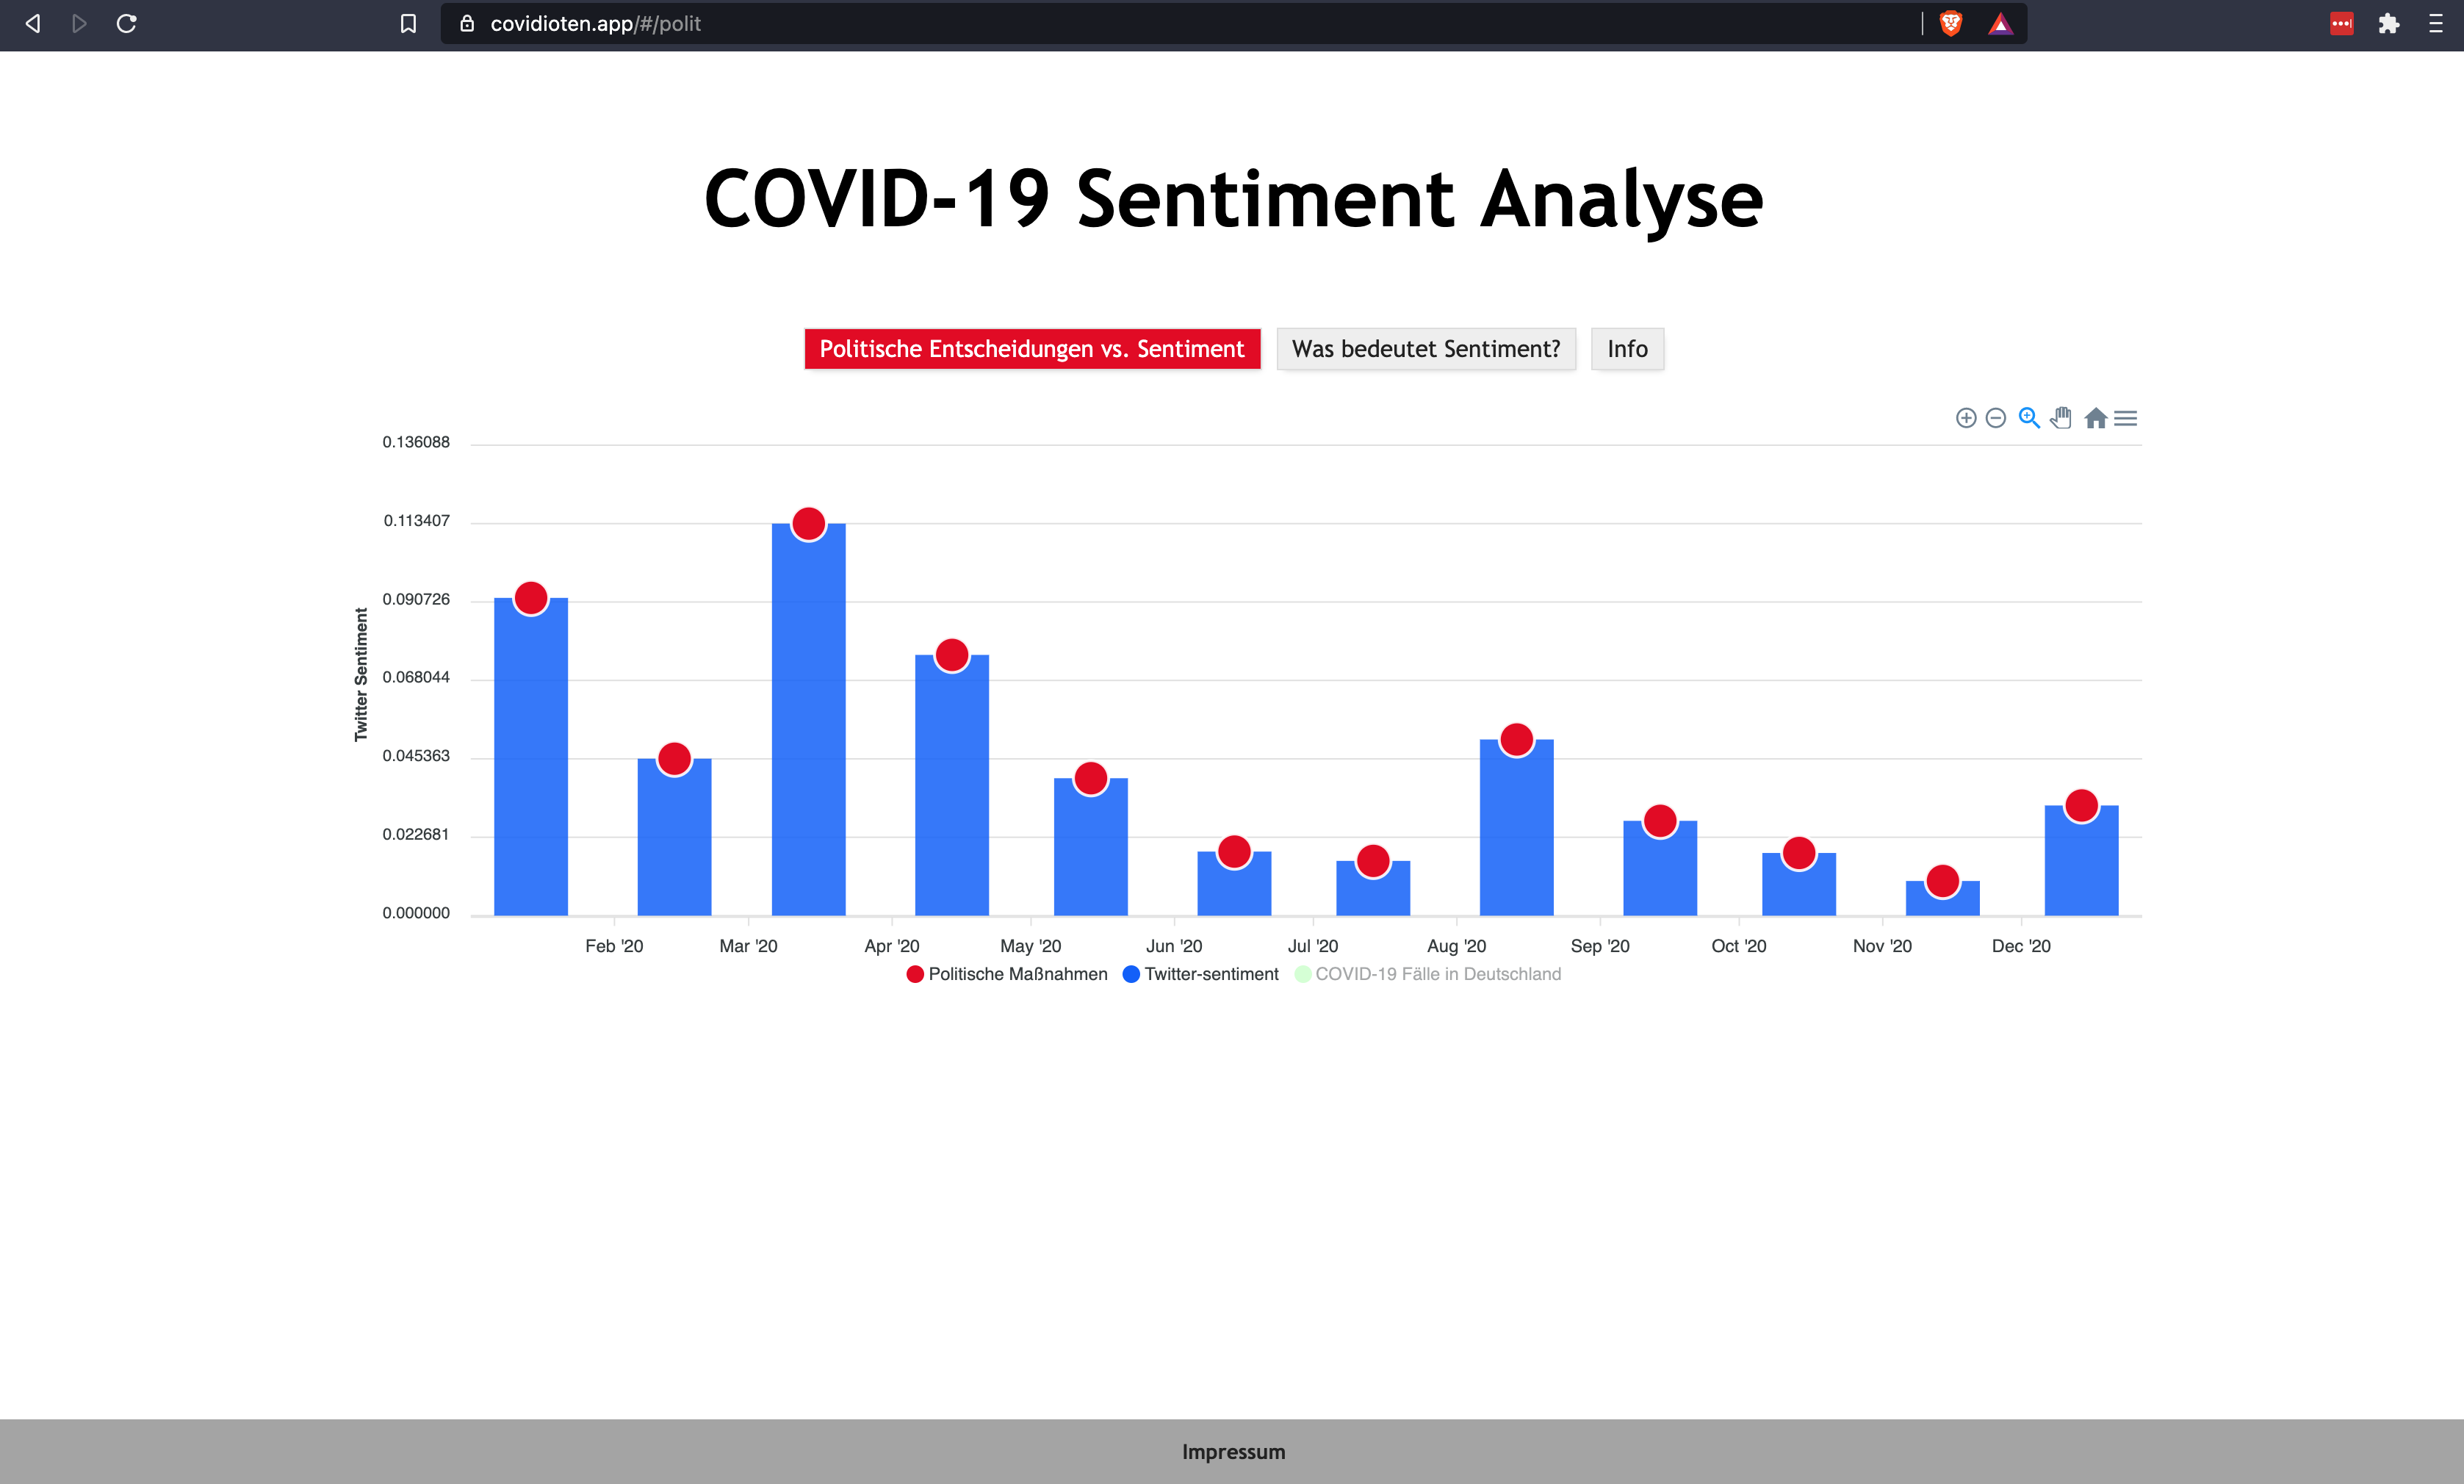
\includegraphics[width=1.0\textwidth]{pic/Disabled_Covid.png}
    \caption{Chart with disabled Covid Cases graph}
    \label{fig:my_label}
\end{figure}

To access the sentiment data in the frontend we used a tool called Axios to create HTTP requests and load the data from an external data base. The active COVID-19 cases and the political measures in Germany were inserted manually as a array and are stored in the frontend. 

\chapter{Conclusion and outlook}
In the last part we want to go over the the things we took from this project as well as what could be done to enhance our app even further. 
We accompanied the whole data science pipeline from running analytic jobs on a cluster of computers over setting up a working software architecture to visualizing data in a comprehensible way. 
The data we used stems from a dataset of Tweets from all over the world from the year 2020. We only used German tweets and calculated the average monthly sentiment. The user interface furthermore provided political information and COVID-19 case numbers that allow the user to notice possible correlations between those data series. For the year 2020, we found that lockdown measures in April were followed by a lower sentiment in May, June and July. Fewer COVID cases in June and July were followed by relaxation of political restrictions and thus a more positive sentiment in August. By providing more up to date data, this analysis could by executed for the year 2021 and even following years. 
\bigbreak
Thanks to this project we had the resources and expertise to get an entry into the field of data science. It was also a good opportunity to get familiar with software development in a group setting including resolving the issues that come with that. Apart from that we also learned a lot about the interpretation of data. For example that you need to be really careful and that you have to consider a big variety of aspects to make reliable statements. And even with a lot of thought on the circumstances it still remains an inherently subjective topic. For example the creator of the sentiment labels has a great impact on the outcome of a sentiment analysis since two people will not perceive and label the same word with the same value. To mitigate the effect of this one could average over the opinions of multiple people to get a general approximation. \\
Furthermore the project gave us an intuition about the algorithms used to determine a text's sentiment. We learned that without expecting industry standard there are easy ways to implement this functionality and frameworks that help you with that.\\
So what else is there to cover? A lot! As already mentioned we only scratched the surface of what is possible and leave a lot of space for improvement. To deepen the understanding of how data is analyzed and get a more reliable result one could use a more sophisticated way of determining the sentiment for example with an artificial neural network. In terms of app functionality the most notable feature to add is to expand the amount of supported languages. Gathering and visualizing more interesting data would be another idea to implement.


\chapter{Links}
\section*{Web Application}
\begin{itemize}
    \item App: \href{https://covidioten.app/#/polit}{covidioten.app}
\end{itemize}
\section*{Github Repositories:}
\begin{itemize}
    \item Public GitHub Organization: \href{https://github.com/Covidioten/}{github.com/Covidioten}
    \item MapReduce and Sentiment Analysis:  \href{https://github.com/Covidioten/BAPraktikumSentimentAnalyse}{github.com/Covidioten/BAPraktikumSentimentAnalyse} 
    \item Backend and Webserver: \href{https://github.com/Covidioten/WebServer}{github.com/Covidioten/WebServer}
    \item Frontend and Visualization: \href{https://github.com/Covidioten/UI}{github.com/Covidioten/UI}
\end{itemize}
\section*{Presentation}
\begin{itemize}
    \item Miro Board: \href{https://miro.com/app/board/o9J_lSwiD0g=/}{miro.com}
    \item Final Presentation: \href{https://docs.google.com/presentation/d/1w5nMCKEQVi0lHkAiSX1hXIUm78zjxiSbUtu0ytRN86I/edit?usp=sharing}{docs.google.com}
\end{itemize}

\section*{Tools and Libraries}
\begin{itemize}
    \item Distributed Computing: \href{https://hadoop.apache.org/}{Apache Hadoop}
    \item Sentiment Analysis: \href{https://hadoop.apache.org/}{TextBlob}
    \item Testing in Python: \href{https://docs.pytest.org/en/6.2.x/}{Pytest}
    \item UML-Sketching: \href{https://plantuml.com/de/}{PlantUML}
    \item API Specification: \href{https://www.openapis.org/}{OpenAPI}
    \item Code Formatting: \href{https://black.readthedocs.io/en/stable/}{Black}
    \item http Requests: \href{https://github.com/axios/axios}{axios}
    \item User Interface: \href{https://vuejs.org/}{Vue.js}
    \item Data Visualization: \href{https://apexcharts.com/}{ApexCharts.js}
    
\end{itemize}

\printbibliography

\end{document}
